\section{Results}
\label{sec:results}

All confirmatory numbers in this section are computed once from hash-locked predictions on the prospective untouched cohort (\nScenes{} scenes; paired scene bootstrap, 95\% CIs) and are machine-read from the locked analysis records into this manuscript.
\Cref{tab:main} reports absolute levels and paired contrasts; \cref{fig:results} plots every primary contrast.

\begin{table*}[t]
  \centering
  \small
  \begin{subtable}{0.44\textwidth}
    \centering
    \begin{tabular}{@{}lccc@{}}
      \toprule
      Arm & Regret $\downarrow$ & Top-1 $\uparrow$ & Pairwise $\uparrow$ \\
      \midrule
      \Lnull{} (scene-blind) & \AbsNullKEightRegret & \AbsNullKEightTopOne & \AbsNullKEightPairwise \\
      \Lgeo{} (incumbent) & \AbsLegacyKEightRegret & \AbsLegacyKEightTopOne & \AbsLegacyKEightPairwise \\
      \Lfull{} (sequence) & \AbsFullKEightRegret & \AbsFullKEightTopOne & \AbsFullKEightPairwise \\
      \Ltok{} (ours) & \textbf{\AbsLasttokenKEightRegret} & \AbsLasttokenKEightTopOne & \AbsLasttokenKEightPairwise \\
      \bottomrule
    \end{tabular}
    \caption{Absolute levels @$K{=}8$ (scene-macro means).}
    \label{tab:main-abs}
  \end{subtable}
  \hfill
  \begin{subtable}{0.53\textwidth}
    \centering
    \begin{tabular}{@{}llll@{}}
      \toprule
      Contrast & $\Delta$Regret $\downarrow$ [95\% CI] & $\Delta$Top-1 $\uparrow$ [95\% CI] \\
      \midrule
      M3: \Ltok$-$\Lnull & \MThreeKEightRegretCI & \MThreeKEightTopOneCI \\
      M2: \Lfull$-$\Lnull & \MTwoKEightRegretCI & \MTwoKEightTopOneCI \\
      M1: \Lfull$-$\Ltok & \MOneKEightRegretCI & \MOneKEightTopOneCI \\
      M5: \Ltok$-$\Lgeo & \MFiveKEightRegretCI & \MFiveKEightTopOneCI \\
      M4: \Lfull$-$\Lgeo & \MFourKEightRegretCI & \MFourKEightTopOneCI \\
      \bottomrule
    \end{tabular}
    \caption{Paired scene contrasts @$K{=}8$ (negative regret / positive top-1 favor the first-named arm).}
    \label{tab:main-delta}
  \end{subtable}
  \caption{\textbf{Main endpoints on the prospective untouched cohort} (\nScenes{} scenes, \nGroups{} groups, 3 seeds). Bold marks the best regret. CIs from paired scene bootstrap ($10{,}000$ resamples). M3 establishes the scene signal (both CIs exclude zero); M1 establishes that the full sequence is \emph{worse} than its last token (both CIs exclude zero); M5 motivates the powered study of \cref{sec:res-incumbent} (both CIs cross zero).}
  \label{tab:main}
\end{table*}

\begin{figure}[t]
  \centering
  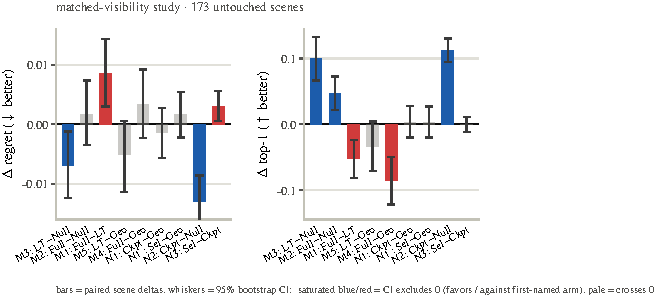
\includegraphics[width=\linewidth]{figs/fig_results.pdf}
  \caption{\textbf{All primary contrasts} ($K{=}8$ selected regret left, tie-aware top-1 right; bars are paired scene deltas, whiskers 95\% bootstrap CIs, drawn directly from the locked analysis records). Saturated blue/red: CI excludes zero, favoring / opposing the first-named arm; pale gray: CI crosses zero. M1--M5: matched-visibility study\iffnonedone; N1--N4: powered incumbent study\else{} (N1--N4 of the powered incumbent study are in flight)\fi.}
  \label{fig:results}
\end{figure}

\subsection{The scene signal is real, and causal}
\label{sec:res-signal}

The paired contrast that isolates scene information---\Ltok{} versus the graph- and parameter-identical scene-blind \Lnull---is CI-supported on \emph{both} co-primary endpoints: selected regret \MThreeKEightRegretCI{} and top-1 agreement \MThreeKEightTopOneCI{} (\cref{tab:main}, M3), on scenes no model in the program had ever consumed.
In absolute terms the last-token selector recovers regret from \AbsNullKEightRegret{} to \AbsLasttokenKEightRegret{} and lifts exact-best agreement from \AbsNullKEightTopOne{} to \AbsLasttokenKEightTopOne; secondary endpoints agree (pairwise ranking accuracy \MThreeKEightPairwiseCI; top-1 at $K{=}5$: \MThreeKFiveTopOneCI, $K{=}2$: \MThreeKTwoTopOneCI).
The effect replicates the direction and magnitude first observed on development scenes during the design phase, making this its first \emph{prospective} confirmation on an untouched cohort.\todo{supp: add the development-phase (E1) record values as the internal-replication table}

Correlation with scene content, not just presence of \emph{some} input, is established by inference-time ablations on the sequence-reading arm (\cref{fig:ablations}): substituting a \emph{different} scene's representation degrades top-1 by \AblWrongSceneTopOneCI, and zeroing it degrades top-1 by \AblZeroSceneTopOneCI---both CIs excluding zero---while regret shifts stay small (\AblWrongSceneRegretCI{} and \AblZeroSceneRegretCI, CIs crossing zero) with no contradictory material improvement on either endpoint.
The degradation concentrating on top-1 is the expected signature: scene content is what disambiguates near-tied candidates at the top of the list.

The full-sequence arm corroborates the signal's existence from a second angle: \Lfull{} also beats \Lnull{} on top-1 (\MTwoKEightTopOneCI, M2)---the sequence \emph{contains} the information---which sharpens the next finding: the failure of \Lfull{} is about \emph{form}, not existence.

\begin{figure}[t]
  \centering
  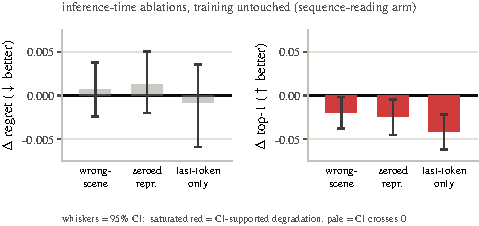
\includegraphics[width=\linewidth]{figs/fig4_ablations.pdf}
  \caption{\textbf{Causal ablations} (inference-time, training untouched; deltas vs.\ the arm's NORMAL condition @$K{=}8$, 95\% CIs). Wrong-scene substitution and zeroing degrade top-1 (CIs exclude zero); the last-token-only diagnostic degrades the \Lfull{} reader (top-1 \AblLastTokenDiagTopOneCI), showing it genuinely consumes sequence positions---yet it still loses to the last-token-trained arm end-to-end (\cref{sec:res-onetoken}).}
  \label{fig:ablations}
\end{figure}

\subsection{One token beats the sequence}
\label{sec:res-onetoken}

Giving the reader the entire $3{,}086\times4{,}096$ prefill---strictly more information than its last row, under an identical parameter budget (\EffParams{} parameters, interchangeable state dicts)---makes selection \emph{worse}, with CI support on both primaries: regret \MOneKEightRegretCI{} and top-1 \MOneKEightTopOneCI{} (\cref{tab:main}, M1).
The deficit is consistent, not a $K{=}8$ artifact: top-1 at $K{=}5$ \MOneKFiveTopOneCI{} and $K{=}2$ \MOneKTwoTopOneCI, pairwise accuracy \MOneKEightPairwiseCI.

Two probes localize the mechanism.
First, the \Lfull{} reader did \emph{not} degenerate into a last-token reader: feeding it only the final row at inference costs it a further \AblLastTokenDiagTopOneCI{} top-1---it genuinely attends across the sequence.
The cost is therefore paid at \emph{training} time: spreading a fixed-capacity reader's cross-attention over 3{,}086 tokens yields a worse selection function than concentrating it on the one token where the generator has already aggregated the scene---the state from which it began emitting candidates.
Second, the auxiliary consequence heads split: \Lfull{} is CI-supported \emph{worse} on future-trajectory ADE (\AuxAdeCI) and collision AUROC (\AuxCollisionCI; $n{=}\AuxCollisionNScenes$ scenes with defined labels) but CI-supported \emph{better} on FDE (\AuxFdeCI).
Sequence access is not uniformly useless---it helps some long-horizon geometry---but the \emph{selection-relevant} summary is best read where the generator itself deposited it.
Under matched parameters, explanations based on reader capacity are excluded by design; what remains is information accessibility.
For practitioners the implication is blunt: the cheapest representation (one token, \EffMemRatio$\times$ less memory than the sequence; \cref{sec:res-eff}) is also the right one.

\subsection{The incumbent test at adequate power}
\label{sec:res-incumbent}

Against the trained geometry incumbent, the matched-visibility study ends in tension (\cref{tab:main}, M5): the representation arm leads on regret (\MFiveKEightRegretCI) while the incumbent leads on exact-best agreement (\MFiveKEightTopOneCI)---absolute top-1 \AbsLegacyKEightTopOne{} vs.\ \AbsLasttokenKEightTopOne---and \emph{both} CIs cross zero.
At $N{=}\nScenes$ this comparison is simply underpowered for the observed effect; concluding either way would be exactly the practice \cref{sec:program} is designed to prevent.
We therefore preregistered a consolidation study sized for it: $N=\FnNTotal$ scenes gives $1-\beta=\FnPowerAchieved$ at two-sided $\alpha=0.05$ for the locked MDE (\FnMde{} regret), with all arms, gates, margins, nomination order, and analysis code frozen before any new scene was scored.

\iffnonedone
\iffnonepass
The nominated representation selector \textbf{passes}: N1 regret \NOneKEightRegretCI{} (CI-supported superiority over \Lgeo) with top-1 non-inferiority satisfied (\NOneKEightTopOneCI{} against frozen margins), and the scene-value contrast replicates at scale (N2 regret \NTwoKEightRegretCI, top-1 \NTwoKEightTopOneCI) on \FnOneNScenes{} scenes.
The checkpoint-objective candidate is reported alongside (N4 regret \NFourKEightRegretCI, top-1 \NFourKEightTopOneCI).
\todo{fill gate-by-gate outcomes + per-cohort consistency clause from the FN1 record; update \cref{fig:results}}
\else
The nominated representation selector \textbf{does not displace the incumbent}: N1 regret \NOneKEightRegretCI{} on \FnOneNScenes{} scenes fails the preregistered superiority gate\todo{state which gate(s) failed, from the FN1 record}, while the scene-value contrast N2 (regret \NTwoKEightRegretCI, top-1 \NTwoKEightTopOneCI) \todo{state whether M3 replicated at scale}.
We report this as a \emph{boundary result} with unusual evidential value: at $0.80$ power, the frozen representation demonstrably adds scene information a geometry selector lacks (\cref{sec:res-signal}, and N2 at scale), yet that information is not sufficient to beat a well-tuned geometry baseline on the promoting endpoint at the effect size that motivated the study.
Representation reuse pays when no tuned incumbent exists or when top-of-list disambiguation (where the scene signal concentrates) is the binding constraint; it does not automatically retire strong geometric priors.
The checkpoint-objective candidate behaves consistently (N4 regret \NFourKEightRegretCI, top-1 \NFourKEightTopOneCI).
\fi
\else
The study is in flight at submission-preparation time: the extension cohort is in acquisition under the frozen protocol, and both outcome branches of this subsection are pre-written against the registered gates. \todo{FN1 finalizes $\sim$Aug 10--11: flip \texttt{\textbackslash fnonedone}/\texttt{\textbackslash fnonepass} in main.tex, run \texttt{make\_numbers.py --fn1}, delete this placeholder paragraph.}
\fi

\subsection{Does the selector loss buy the top of the list?}
\label{sec:res-selloss}

The controlled contrast N3 isolates the objective of \cref{eq:selloss}: same architecture, same data, rank term replaced by the regret-weighted best-vs-rest logistic.
The preregistered success criterion is asymmetric by design---the selector loss must \emph{buy} top-1 (CI above zero) without \emph{selling} regret (CI upper bound below $+0.005$)---because the design-phase precedent showed a large top-1 gain (${\sim}{+}0.08$) at a small regret concession.\todo{supp: cite exact E1 record values}
\iffnonedone
N3 lands at top-1 \NThreeKEightTopOneCI{} and regret \NThreeKEightRegretCI: \iffnonepass the trade clears the gate, and the selector-objective candidate is the nominated arm reported above.\else\ \todo{write the observed verdict: gate cleared / not cleared, and which candidate was nominated}\fi
\else
\fnpending
\fi

\subsection{Efficiency}
\label{sec:res-eff}

\Cref{tab:eff} summarizes deployment cost on a single workstation GPU.
The deployed configuration---last token in, all $K{=}8$ candidates scored---runs in \EffLtMedianMs{}\,ms median (\EffLtTailMs{}\,ms p95) with \EffLtMemMb{}\,MB peak incremental memory and \EffParams{} trainable parameters, orders of magnitude under the preregistered ceilings (\EffCeilMedianMs/\EffCeilTailMs\,ms, \EffCeilMemGb\,GiB, \EffCeilParams{} params).
The representation itself is free: it is a byproduct of the prefill that generates the candidates.
No VLA finetuning, no world model, no inference-time rollouts; the entire selector trains in minutes (peak \EffTrainPeakMb\,MB per worker).
For contrast, the full-sequence reader needs \EffFullMemMb{}\,MB at inference (\EffMemRatio$\times$ more) and is \emph{worse} (\cref{sec:res-onetoken}); explicit-imagination designs additionally pay for a purpose-trained world model and its inference-time rollouts, a cost class our amortized route avoids entirely.

\begin{table}[t]
  \centering
  \small
  \begin{tabular}{@{}lrrr@{}}
    \toprule
    & Params & Latency (med/p95) & Peak mem \\
    \midrule
    \Ltok{} head (deployed) & \EffParams & \EffLtMedianMs{}/\EffLtTailMs{}\,ms & \EffLtMemMb{}\,MB \\
    \Lfull{} reader & \EffParams & \EffFullMedianMs{}/\EffFullTailMs{}\,ms & \EffFullMemMb{}\,MB \\
    \midrule
    Preregistered ceiling & \EffCeilParams & \EffCeilMedianMs{}/\EffCeilTailMs{}\,ms & \EffCeilMemGb{}\,GiB \\
    \bottomrule
  \end{tabular}
  \caption{\textbf{Deployment cost} (incremental over the generator, all $K{=}8$ candidates, bf16, single workstation GPU; 200 timed iterations).}
  \label{tab:eff}
\end{table}

\iffnonepass
\subsection{Sealed-cohort confirmation}
\label{sec:res-sealed}
Following promotion, the 35-scene sealed cohort---never opened by any stage of the program---was unsealed exactly once. \todo{FN2: fill when/if it exists.}
\fi
